\section{Datasets}
\label{sec:datasets}
The experiments will be conducted on two different aerial image datasets. The first is provided by Minh. The performance can be compared to other works. The second dataset have been created from publicly available sources by the author of this thesis. Differences and similarities of these datasets will be further discussed below. \\

\textbf{Massachusetts Roads Dataset}
(Write stats, show example)
\textbf{Massachusetts Buildings Dataset}
\todo[inline]{Include or not?}
\textbf{Norwegian Roads Dataset}
This dataset presents some challenges in terms of label resolution. Road labels registration errors. Fewer omission errors.
Road labels not generated with uniform breadth. Road labels more accurate in terms of road breadth. Images taken mainly from urban and suburban areas throughout norway. In terms of typograhy (Right word?). Cultivated land, mountains, ice, forest areas. Images also range in quality. Different color hues. Vegvesenet --
Ground sampling distance of 0.66. 
The dataset covers an area of approximately 
1200 km2.\\

In addition to the Massachusetts Roads Dataset \citep{MnihThesis}, the proposed algorithm will be tested on a new dataset. This dataset was constructed from aerial images retrieved from Kartverket, which depicts both rural and urban areas in Norway. The labels for this dataset have been generated from road center-line vectors found in the publicly available topographic vector database, N50, provided by Kartverket. \\

Currently, the dataset contains 221 RGB images that are 1536 pixels in width and height. The images have a high resolution with a \ac{GSD} of around 0.66 meters per pixel. There are 184 images in the training set, 21 images in the validation set, and 16 images in the test set. The road center-line vectors are generated as 4 pixel wide black lines in the label images. A cropped image from this dataset can be seen in Figure \ref{fig:aerialimage_norwegian}, with the label image superimposed on the aerial image. Observe that some roads are missing from the label image, as well as the ground truth not covering the roads properly. \\

\begin{figure}[t]
\begin{center}
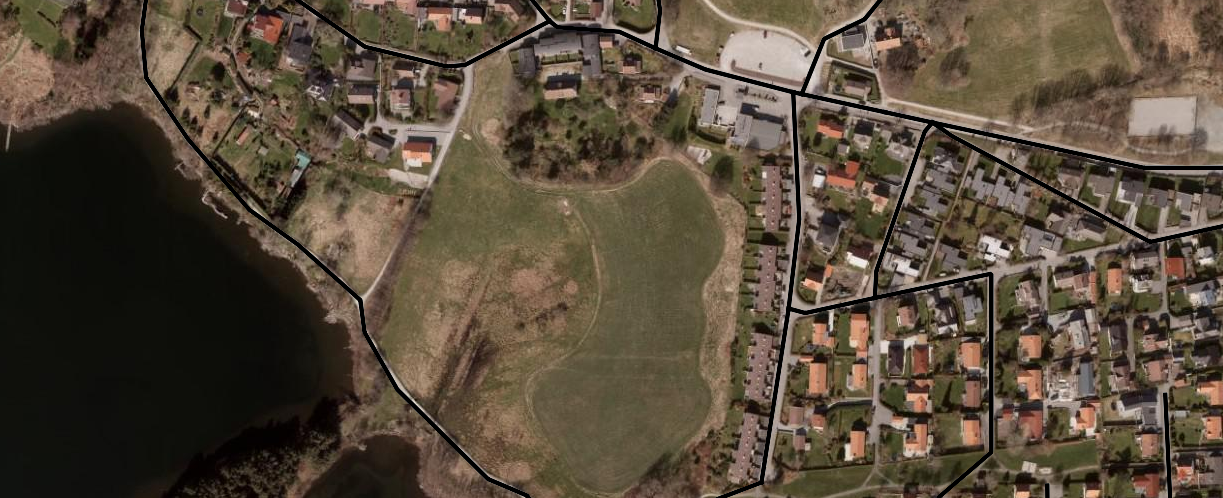
\includegraphics[width=1\columnwidth]{figs/norwegian_dataset.png}
\caption[Norwegian road dataset example]{Example aerial image with the label image as an overlay.}
\label{fig:aerialimage_norwegian}
\end{center}
\end{figure}

The Norwegian Roads Dataset has been constructed by using QGIS, an open source geographic information system application. The application enables viewing and editing of map data, but also provides a Python interface. A script to create label images was developed, which takes the map coordinates associated with each corner of an aerial image, and generates a raster image of road center-line vectors found inside that area. These raster images can be used as label data in supervised learning. \\